%% FEUP THESIS STYLE for LaTeX2e
%% how to use feupteses (English version)
%%
%% FEUP, JCL & JCF, 31 July 2012
%%
%% PLEASE send improvements to jlopes at fe.up.pt and to jcf at fe.up.pt
%%

%%========================================
%% Commands: pdflatex tese
%%           bibtex tese
%%           makeindex tese (only if creating an index)
%%           pdflatex tese
%% Alternative:
%%          latexmk -pdf tese.tex
%%========================================

\documentclass[11pt,a4paper,twoside,openright]{report}

%% For iso-8859-1 (latin1), comment next line and uncomment the second line
\usepackage[utf8]{inputenc}
\usepackage{subcaption}
\usepackage{amsmath}
\usepackage{float}
\usepackage{lscape}
\usepackage{textcomp}
\usepackage{pgfgantt}
%\usepackage[latin1]{inputenc}

%% English version

%% MIEIC options
%\usepackage[mieic]{feupteses}
%\usepackage[mieic,juri]{feupteses}
%\usepackage[mieic,final]{feupteses}
%\usepackage[mieic,final,onpaper]{feupteses}

%% MIEEC options
\usepackage[mieec]{feupteses}
%\usepackage[mieec,juri]{feupteses}
%\usepackage[mieec,final]{feupteses}

%% For other degrees
%\usepackage{feupteses} % you must define the degree bellow

%% Additional options for feupteses.sty: 
%% - onpaper: links are not shown (for paper versions)
%% - backrefs: include back references from bibliography to citation place

%% Uncomment to create an index (at the end of the document)
%\makeindex
\graphicspath{{figures/}}

%%----------------------------------------
%% TIP: if you want to define more macros, use an external file to keep them
%some macro definitions

% format
\newcommand{\class}[1]{{\normalfont\slshape #1\/}}

% entities
\newcommand{\Feup}{Faculdade de Engenharia da Universidade do Porto}

\newcommand{\mc}[1]{\mathcal{#1}}
\newcommand{\mb}[1]{\mathbf{#1}}

%%----------------------------------------

%%========================================
%% Start of document
%%========================================
\begin{document}

%%----------------------------------------
%% Information about the work
%%----------------------------------------
\title{Dissertation Preparation}
\author{José Pedro Castro Fonseca}

%% Comment next line if not necessary for degree
\degree{Integrated Masters in Electrical and Copmuter Engineering}

%% Uncomment next line for date of submission
%\thesisdate{July 31, 2008}

%% Comment next line copyright text if not used
\copyrightnotice{José Fonseca, 2016}

\supervisor{Supervisor}{João Canas Ferreira}
\supervisor{Second Supervisor}{Ivo Timóteo}

%% Uncomment next line if necessary
%\supervisor{Second Supervisor}{Name of the Supervisor}

%% Uncomment committee stuff in the final version if used
%\committeetext{Approved by \ldots:}
%\committeemember{President}{Name of the President}
%\committeemember{Referee}{Name of the Referee}
%\committeemember{Referee}{Name of the Referee}
%\signature

%% Specify cover logo (in folder ``figures'')
\logo{uporto-feup.pdf}

%% Uncomment next line for additional text below the author's name (front page)
%\additionalfronttext{Preparação da Dissertação}

%%----------------------------------------
%% Preliminary materials
%%----------------------------------------

% remove unnecessary \include{} commands
\begin{Prolog}
  \cleardoublepage
  \pdfbookmark[0]{Table of Contents}{contents}
  \tableofcontents
  \cleardoublepage
  \pdfbookmark[0]{List of Figures}{figures}
  \listoffigures
  \cleardoublepage
  \pdfbookmark[0]{List of Tables}{tables}
  \listoftables
  \chapter*{Abbreviations and Symbols}
%\addcontentsline{toc}{chapter}{Abbreviations}
\chaptermark{Abbreviations and Symbols}

\begin{flushleft}
\begin{tabular}{l p{0.8\linewidth}}
ANN      & Artificial Neural Networks\\
BPTT     & Backpropagation Through Time\\
CNN      & Convolutional Neural Network\\
CPU      & Central Processing Unit\\
FPGA     & Field-Programmable Gate Array\\
LSTM     & Long Short-Term Memory\\
RNN      & Recursive Neural Networks\\
SPSA     & Simultaneous Perturbation Stochastic Approximation\\
\end{tabular}
\end{flushleft}

  % the list of abbreviations used
\end{Prolog}

%%----------------------------------------
%% Body
%%----------------------------------------
\StartBody

%% TIP: use a separate file for each chapter
\chapter{Introduction}\label{chap:intro}
Brief overview of the report:

In Chapter~\ref{chap:intro}, I will present a conceptual background to the problem at hand, exposing the background that surrounds it~\ref{sec:intro_back}, the motivation for the desired solution~\ref{sec:intro_mot}, its objectives~\ref{sec:intro_obj} and, lastly, the people that will help me achieve them~\ref{sec:intro_people}.

In Chapter~\ref{chap:theorBack}, the theoretical foundations will be layed out. Section~\ref{sec:tb_basicCon} presents the basic concepts of Machine Learning, and in the following sections, the theoretical details of ANNs, RNNs and LSTMs. Section~\ref{sec:training_lstm} provides a quick explanation of the training algorithm that will be used in the final solution, which will be outlined in Section~\ref{sec:propSol}.

In Chapter~\ref{chap:workPlan}, the work plan for the Dissertation work is detailed as \emph{tasks} in Section~\ref{sec:wp_tasks_td}, and their temporal arrangement is pictured in a Gantt chart in Section~\ref{sec:wp_tasks_gantt}. Furthermore, the description of the Hardware and Software resources that I will be utilizing during the course of my work is done in Section~\ref{sec:wp_sh}

In Chapter~\ref{chap:stateArt}, the state of the art of LSTMs, their applications~\ref{sec:sa_apps}, their hardware implementations~\ref{sec:sa_hardware} and the current work regarding the chosen training algorithm~\ref{sec:sa_training} are presented.

Finally, in Chapter~\ref{chap:earlyWork} I will present some of the work that I have already concluded.

\section{Background}\label{sec:intro_back}
Artificial Neural Networks are one of the most popular models in the field of Machine Learning. As the name suggests, their operation is inspired by the operation of the building blocks of our brain, the \textbf{neurons}. In spite of its high performance, one of their shortcomings is the fact that they cannot retain temporal dependences among incoming data samples, thus not being suitable to process time-series data, such as audio, video or other kinds of time-varying data streams, where current inputs have a high temporal dependence with previous and future inputs. 

To address this issue, several algorithms have been used, such as Hidden Markov Models (HMM) or Recurrent Neural Networks (RNN), but both of these methods fail to recall temporal dependences that extend over an large period of time, for the reasons that we will understand in Sections~\ref{sec:theorBack_rnn} and~\ref{sec:theorBack_lstm}.Thus, in 1997 Hochreiter et al. proposed a novel RNN structure~\cite{Hoch97}, the Long Short-Term Network (LSTM), where a memory cell was introduced, and the input/output/read/write access is controlled by individual gates that are activated both by the incoming data samples, but also by the outputs from the previous time-step (it is an RNN after all). They are one of the state of the art methods in Deep Learning nowadays, as we can attest in Section~\ref{sec:sa_apps}.

\section{Motivation}\label{sec:intro_mot}
Hitherto, and to the best of my knowledge, all of the published applications that use LSTM are software based, but the parallel nature of the structure hollers for a dedicated hardware realization that can dramatically increase its performance, something that  has only recently been done once~\cite{Chang15} (see Section~\ref{sec:sa_hardware} for further details), and although it improves the processing time when compared to a naïve software solution, it still lacks the ability to perform on-chip learning, and the learning process is performed offline, in a normal CPU, when it also could be sped up by a dedicated hardware structure.

All these techniques are generally implemented in mainstream processors, making use of general high-level or low-level languages, where all the real parallelism is limited to the number of simultaneous threads that we can run on each physical core, which up to now generally have between 2-8 cores (mobile devices and general use personal computers), 

In order to parallelize the computations to the fullest extent, a solution is to port it both to a Graphics Processing Unit (GPU) or even a Field-Programmable Gate Array (FPGA), but the porting process is not entierely automatic and to have the least performance drop possible, it has to be explicitly programmed in CUDA/OpenCL for GPUs, and a Hardware Description Language for FPGAs, with an increasing level of complexity and low-level details. Therefore, it is necessary to provide frameworks that can allow an FPGA to quickly reconfigure itself to run these kind of networks on demand, for a particular task that requires them, achieving a lower computation time, and unburdening the CPU from running it, thus saving performance for running other tasks related with the Operating System, for instance. Furthermore, when processing an incoming stream of highly dimensional data, or with high throughput, a CPU solution might not be scalable, and could benefit greatly from a dedicated hardware implementation.

\section{Objectives}\label{sec:intro_obj}
Taking into account the considerations done in~\ref{sec:intro_mot}, I propose to develop a hardware implementation of an LSTM Network, \emph{with on-chip learning}, improving the performance, capability and flexibility of the existing solution of~\cite{Chang15}. Moreover, I also propose to benchmark this solution and try to compare it with the software performance results of~\cite{Tavear13} and, as a secondary objective, try to use my developed structure to replicate some of the applications portrayed in~\ref{sec:sa_apps}. Lastly, I will work to make this structure reconfigurable on the go, and trying to minimize the reconfiguration time.

\section{People Involved}\label{sec:intro_people}
Besides me, the candidate to the Master's Degree, there are two more people involved, namely

\begin{itemize}
    \item \textbf{Supervisor} -- The \href{https://sigarra.up.pt/feup/pt/func\_geral.formview?p\_codigo=210963}{Professor João Canas Ferreira}, auxiliary professor at the Faculty of Engineering of the University of Porto.
    \item \textbf{Second Supervisor} -- \href{http://www.cl.cam.ac.uk/~ijpdmt2/}{Ivo Timóteo}, MSc, a Computer Science PhD candidate at Cambridge University, UK, in the field of Artificial Inteligence.
\end{itemize}


\chapter{Theoretical Background}\label{chap:theorBack}


\section{Basic Concepts of Machine Learning}
Machine Learning is a field of Computer Science that studies the development of mathematical techniques that allow software to learn autonomously, without an explicit description of each rule of operation. Its goal is to extract latent features from the data that allow an immediate classification of each input data into a particular class -- the catch is that there is no previous rule formulation, but instead we have an adaptive model that adjusts is parameters accordingly with the input data it receives, improving the estimates it yields as it receives new input samples. 

Let us consider a practical example. For instance, suppose we want to build a program that given an input audio waveform representation of a spoken word, it matches it into a particular word of a dictionary. We could, of course, devise a set of rules and exceptions for each word analysing some of its features (perhaps the Fourier representation of each one, and, from it, manually finding the appropriate rules for each), but apart from it being a very complex task, it wouldn't be a scalable solution, given the enormous number of words in each language. The approach taken by Machine Learning is diametrically different, and instead of manually processing each waveform, we build a large dataset, of size $N$, containing the waveforms of several words $\left[ \mb{x}_1 \; \mb{x}_2 \;\mb{x}_2 \; \dots \mb{x}_N \right]$ -- we call this dataset the \textbf{training dataset} -- and we feed it to our model. Each of the $i$-th data point was previously labelled, and in fact we feed each training data point $\mb{x}_i$ \emph{along} with its corresponding label $t_i$, so that the model can adapt its parameters accordingly to the \emph{target value} it is supposed to classify. This set of labels $\mb{t} = \left[ t_1 \; t_2 \; t_3 \; \dots \; t_N \right]$ is called the \textbf{target vector}. 

We are, then, left with the following question: how can the model quantitatively evaluate the quality of its current set of parameters? That could be achieved in a number of ways, but the most usual is using a \textbf{Cost Function} that, as the name suggests, measures the cost of each wrong classification of the model. The model then evolves in a way that minimizes the cost function. A usual choice for the cost function is the \textbf{sum of squares error}. Mathematically, if $y_{\theta}^i = y_{\theta}(x_i)$ is the prediction for the input data point $x_i$ with label $t_i$, given the current set of parameters $\theta$, the cost function using this metric is given by

\begin{equation}\label{eq:costfunctionFund}
	J(\theta) = \frac{1}{2} \sum_{i=1}^N \left( y_{\theta}^i - t_i \right)^2.
\end{equation}

Sometimes, instead of applying the raw data to the model, we can apply some sort of \emph{preprocessing} to the data to extract the relevant features from it. For instance, instead of just feeding a raw image, we can perform several operations like edge detection or low-pass filtering, and apply them in parallel. In cases of highly dimensional data (i.e. each data vector has a very high number of features), we can apply techniques like \textbf{Principal Component Analysis} to reduce the feature space to a smaller dimension one, where the previous features were combined into two or three new features that pose themselves as the most relevant.

The problems described above are, in fact, a subset of the problems that Machine Learning tries to address. These problems are called \textbf{classification problems}, because for each input data point, our model tries to fit it into the most appropriate class. But we can also address \textbf{regression problems} where the output is not limited to a discrete set of values but rather a continuous interval. On the other hand, the Neural Network that this work will implement addresses a special kind of classification problem, where the classification decision is influenced not only by the current input sample, but also by a given \emph{window of samples} that trail the current sample.

In summary, the most typical setting for a Machine Learning problem is having a large \textit{input dataset} which we use to \textit{train} our model (i.e. allowing him to dynamically adapt its set of parameters $\theta$), in order to produce an output label $y_i$ for each of them that minimizes a quality metric, the \textit{Cost Funcion}, which can be chosen to the sum of squared differences, the log-loss, or any other appropriate  mathematical relationship  between the estimate $y_i$ and the correct label $t_i$. 

Now that the basic Machine Learning concepts have been presented, I will discuss, henceforth, one of the most important algorithms that address the supervised classification problems, the \emph{Artificial Neural Networks} that will be discussed in Section~\ref{sec:theorBack_ann} as somewhat of a contextual introduction to the main theme of the thesis, which will be Recurrent Neural Networks (Section~\ref{sec:theorBack_rnn}), namely the \textbf{Long Short-Term Memory Networks} (Section~\ref{sec:theorBack_lstm}), both of which are improvements over the initial formulation of the ANNs. These two last networks branch even further from these set of problems, and are usually employed in \textit{Deep Learning} tasks, where we try to extract even higher level information from data at the expense of increased model complexity. 

\section{Artificial Neural Networks}\label{sec:theorBack_ann}

Artificial Neural Networks (ANN) are mathematical structures that, as the name suggests, try to mimic the Human Brain. ANN's building blocks, like their biological counterpart, model the high-level behaviour of biological neurons, in the sense that they neglect unnecessary biological aspects (such as modeling all the voltages across the neuron and all its electromagnetic interactions), and only retain its fundamental underlying mathematical function, which is a weighted linear combination of its inputs subject to a \emph{activation function}, i.e. a function that outputs a decision value depending on its inputs.  Mathematically, we have

\begin{equation}
	y = f(\mb{w}^T \mb{x} + b_0)
\end{equation}
where $\mb{w} = \left[ w_1 \; w_2 \;  w_3 \;  \dots \; w_n \right]$ is the input weight vector, $\mb{x} = \left[ x_1 \; x_2 \; x_3 \; \dots \; x_n \right]$ the input vector, $b_0$ is the bias factor and $f(\cdot)$ is the chosen activation function. Furthermore, we call the scalar quantity $a = \mb{w}^T \mb{x} + b_0$ the \textbf{activation}, since its value determines how the activation function will behave. Figure~\ref{fig:modelNeuron} exemplifies the roles of these variables within our neuron model, and compares each part of it with the biological counterpart.

\begin{figure}[!H]
	\begin{subfigure}{0.5\linewidth}
		\centering
		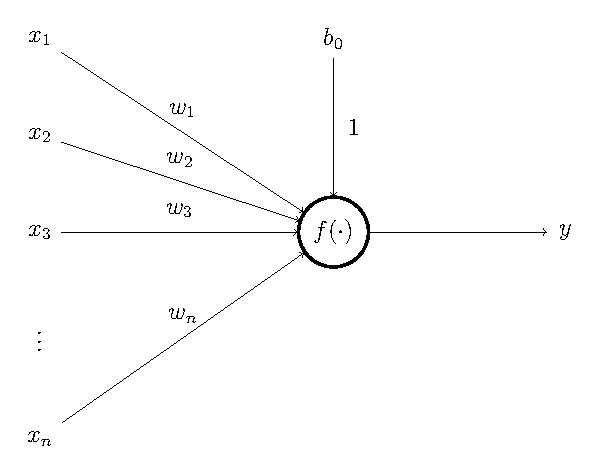
\includegraphics[width=0.9\linewidth]{figures/neuron.eps}
		\caption{Neural Network Node}
		\label{fig:modelNeuron_a}
	\end{subfigure}
	\begin{subfigure}{0.5\linewidth}
		\centering
		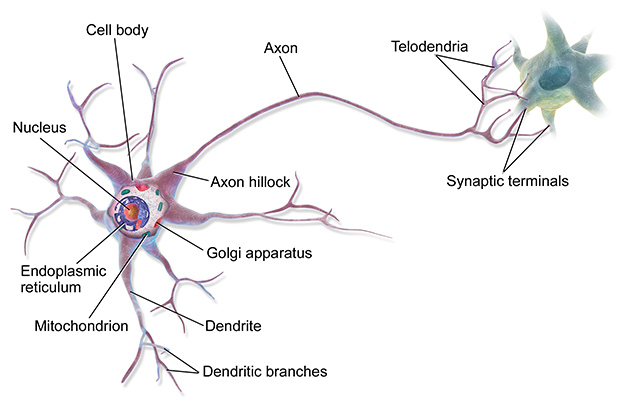
\includegraphics[width=0.9\linewidth]{figures/multipolarNeuron.png}
		\caption{Biological Neuron Diagram}
		\label{fig:modelNeuron_b}
	\end{subfigure}
		
	\caption{In Figure~\ref{fig:modelNeuron_a}. each input feature $x_i$ is weighted by its corresponding weight $w_i$. During the training procedure, these weights are adjusted so that the output $y$ approaches the target value. In Figure~\ref{fig:modelNeuron_b}, we see the diagram of an actual multi polar neuron. The dendrites, where the stimuli are received, plays a role similar to that of the input nodes. The axon transmits the signal to the synaptic terminals, that are similar to the $y$ output}
	\label{fig:modelNeuron}
\end{figure}


As far as the activation function is concerned, we can have several types. An immediate choice would be the \textbf{Binary Step Function} that  outputs -1 if the activation is \textbf{below} a given threshold and 1 otherwise. There can also be \textbf{real valued activation functions}, whose output is not binary, but rather that of a continuously differentiable function, such as the logistic sigmoid $\sigma(a) = \frac{1}{1 + \mathrm{e}^{-a}}$ or the hyperbolic tangent $\tanh(a)$. This aspect will prove useful for the usual training methods, that involve the computation of derivatives. In Figure~\ref{fig:activFunc} these activation functions are plotted.

\begin{figure}[H]
	\centering
	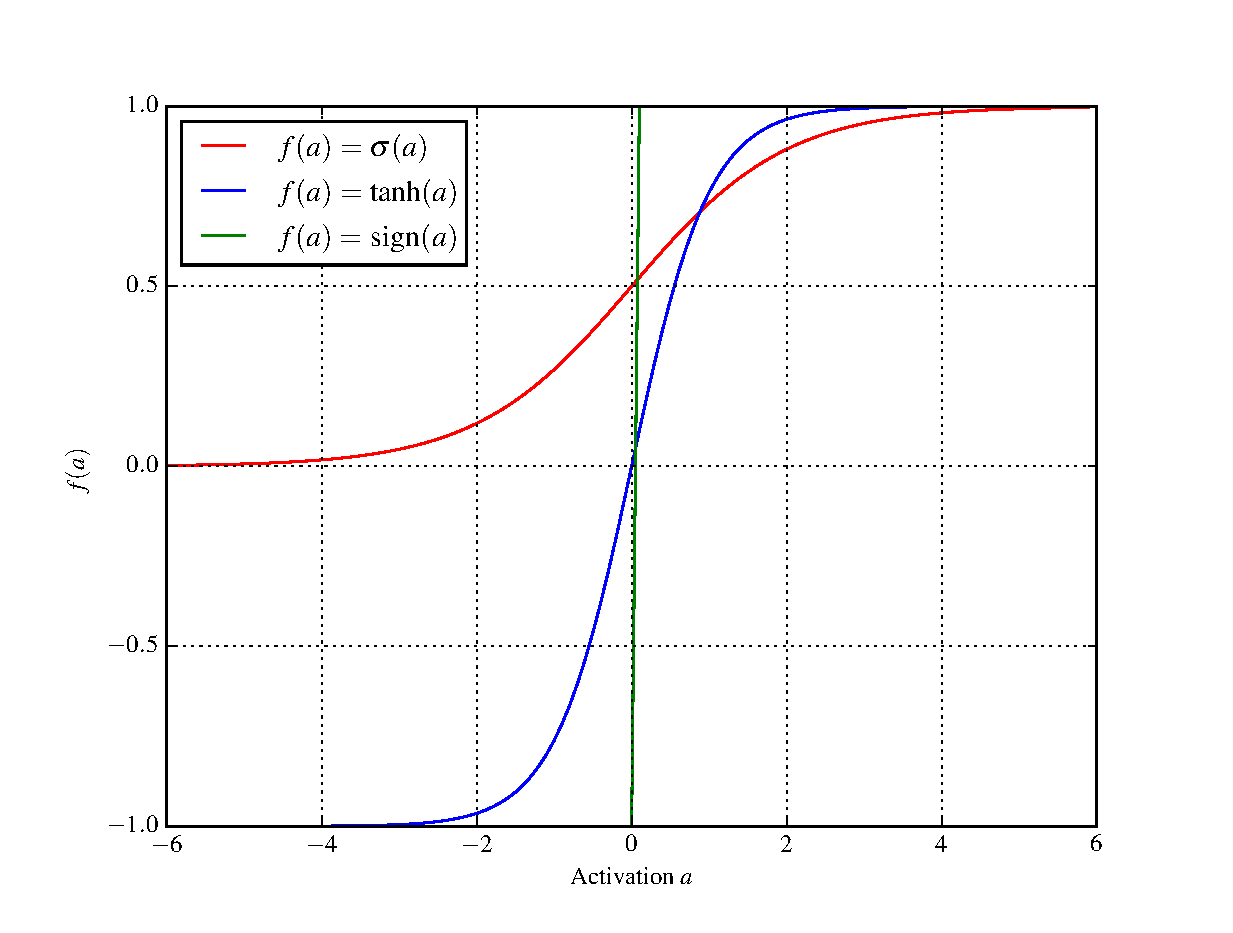
\includegraphics[width=0.9\linewidth]{figures/activFunc.eps}
	\caption{Three different activation functions. As you can see, the hyperbolic tangent has the same extreme value as the sign step function, but has a smooth transition between them, which can be interpreted as a \emph{soft decision} in the more ambiguous middle region, reflecting the degree of uncertainty on the decision. On the other hand, the sigmoid function goes from zero to one, and is also smooth like the hyperbolic tangent}.
	\label{fig:activFunc}
\end{figure}


A neuron by itself can be thought of as a simple linear regression, where we optimize the weight of each feature according to a target value, or function. While important in some applications, the main interest in ANN is to evaluate increasingly more complex models, and not a simple linear regression. This is achieved by \emph{chaining} nodes to one another, connecting the output of a given node to one of the inputs of another. We call \emph{layers} to a group of these nodes that occupy the same hierarchical position. There can be any number of layers, with any number of nodes, but most implementations generally have 3 layers: the \emph{initial} layer, the \emph{hidden} layer (in the middle) and the \emph{output} layer. Figure~\ref{fig:neuralnet} suggests a possible structure for a 3 layer ANN. 


\begin{figure}[H]
	\centering
	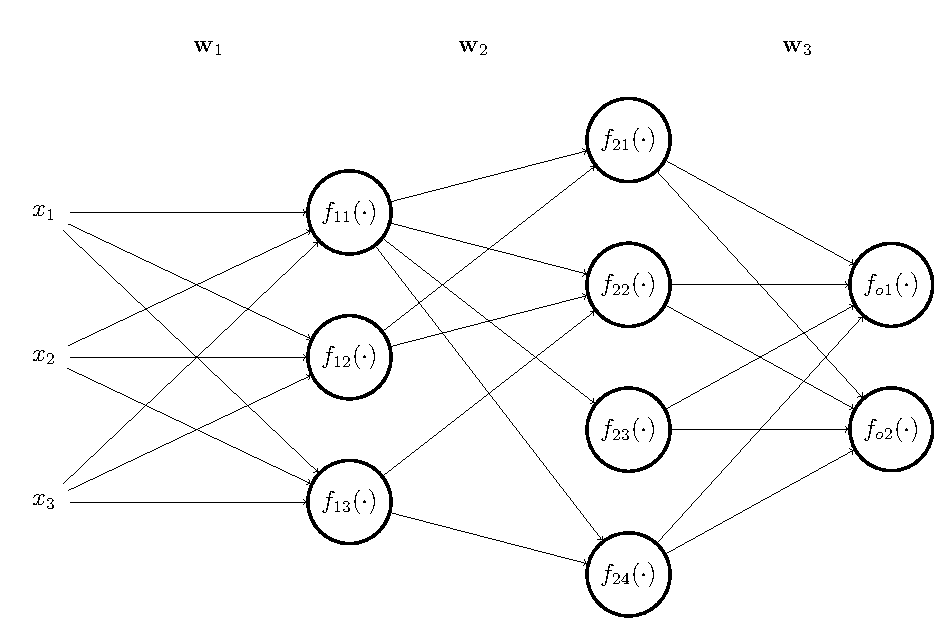
\includegraphics[width=0.9\linewidth]{figures/ann.eps}
	\caption{A three layer ANN. We have omitted some of the connections in the hidden layer, for simplification purposes. $\mb{w}_1$ represents the weight matrix of the input layer, $\mb{w}_2$ the weight matrix of the connections between the input layer and the hidden layer, and $\mb{w}_3$ the weight connections between the hidden and the output layer. $f_{ij}(\dots)$ is the activation function of the $j$-th neuron of the $i$-th layer. Since they can be different, I chose different indexes to each.}
	\label{fig:neuralnet}
\end{figure}

Regarding the training of ANNs, is is performed through a two-step process: first, a \textbf{feed-forward} step where the input is applied, and the activations are evaluated in succession up to the output neurons; then, the perform the \textbf{backpropagation} step, where we calculate the errors in each of the nodes, but now from the output to the input: the weights are updated and optimized using an iterative  method called \textit{Gradient Descent}, where if $\tau$ is the current time step, the next update on the weight matrix $\mb{w}^{(\tau+1)}$ is given by

\begin{equation}\label{eq:gradDesc}
	\mb{w}^{(\tau+1)} = \mb{w}^{(\tau)} - \eta \nabla E(\mb{w}^{(\tau)})
\end{equation}
where $E(\cdot)$ is the error function. As we can see, the weight matrix is moved in the direction that minimizes the error function the most, and $\eta$ controls how fast this is achieved, being the reason why it is called the \textbf{learning rate}.

The computation of gradient of the error function comprises the evaluation of its derivatives with respect to each weight of all network connections, $w_{ij}$. They are

\begin{equation}\label{eq:partialE}
	\frac{\partial E}{\partial w_{ji}} = \delta_j f(a_i)
\end{equation}
where $f(\cdot)$ is the activation function of the neuron and

\begin{equation}\label{eq:deltaj}
	\delta_j = f'(a_j) \sum_k w_{kj} \delta_k .
\end{equation}
The interpretation of these equations is simple. If $w_{ji}$ is the weight of the connection between the neuron $j$ we are considering and a neuron $i$ in a previous layer, then the sum over $k$ relates to all the neurons in the \emph{next} layer to which $j$ connects: this way, since the update on $w_{ji}$, according to~\ref{eq:gradDesc}, is given by

\begin{equation}\label{eq:update}
	w_{ji}^{(\tau+1)} = w_{ji}^{(\tau)} - \eta \frac{\partial E}{\partial w_{ji}}
\end{equation}
we see that, from~\ref{eq:partialE}  it simply is the product of the error of the current neuron, $\delta_j$, with the output of the previous neuron $f(a_i)$. In turn, from~\ref{eq:deltaj}, we see the recurrence relationship between it and the weighted sum of all posterior neurons that connect to it. Hence, the name backpropagation is now clear: we are, in fact, propagating the errors backwards into the neuron of interest, weighted by the corresponding weight, but now \emph{backwards} instead of forward, as before. For the output units, the $\delta_j$ is simply the difference between the produced output and the corresponding label for that sample. This two-step process is performed for every data point in out dataset. %%Place where I can include an algorithmic overview?
For a complete proof of the above formulas, see~\cite[chap. 5.3.1]{Bishop2006}.

\section{Recurrent Neural Networks}\label{sec:theorBack_rnn}
A Recurrent Neural Network (RNN) is, essentially, a regular ANN where some neurons (especially in the hidden layer) have \emph{feedback connections} to themselves, i.e. their outputs are fed as inputs. The relevance of this different structure is the possibility to retain \emph{sequence} information about the data. Before, each incoming data point only contributed to the training of the network, but no information about the correlation between themselves and the data points that preceded them did not influence the training step. They were regarded as if no temporal relationship existed, and therefore each data point is conditionally independent of any other. This is obviously not necessarily truth, and in fact there are many cases, where the correlation between data points is high for those closely spaced in time, in which it is actually completely false, as in video signals, audio signals, or other kinds of \emph{temporal sequences} of data. Therefore, the feedback connection of the neuron to himself acts as a kind of \emph{memory element} that takes into account in the present decision, the history of decisions previously taken, and hence the previous data. 
Figure~\ref{fig:recneuron} suggests a possible structure for a neuron of a hidden layer in an RNN, and also an alternate representation, where the structure is unfold through time.

%% METE AQUI A FIGURA

The training of an RNN is usually performed using a variation of Backpropagation, called \textbf{Backpropagation Through Time} (BPTT), that as the name implies, performs the same backpropagation procedure discussed for the ANNs, but now taking into account the unfolding of the network through a fixed training epoch $T$ like Figure~\ref{fig:recneuron}. Due to this very fact, this training procedure is memory and performance consuming, and so it will not be used in my final work, but instead a novel approach, the \textbf{Simulatneous Perturbation Stochastic Approximation}. 

Even though RNNs outperform static ANNs in sequence recognition problems~\cite{Bengio1991}, they fail to retain long-term dependencies. Of course that the weight training process is itself a form of memory, but the problem is that the weight update is much slower than the activations~\cite{Yoshua01}, and therefore this memory only retains short-term dependencies. This is because of the so-called \textbf{Vanishing Gradients Problem}~\cite{Yoshua94,Yoshua01}, where the error decays exponentially through time, and the impact of previous incoming data points on the training of the weights, and thus the current decision, quickly decreases. 


\section{Long Short-Term Memory Networks}\label{sec:theorBack_lstm}
To overcome the issue of failing to remember long-term dependencies, Hochreiter and Schmidhüber proposed, in 1997, a novel approach to the RNNs called the \textit{Long-Short Term Network}~\cite{Hoch97}. This section explains the main idea of this approach~\ref{sec:struct_lstm}, and also how it is trained\ref{sec:training_lstm}, serving as a support basis for the work of this thesis.
Although originally formulated in 1997, its formulation has been incrementally updated in~\cite{Gers00} and~\cite{Gers2000}, and the most current version is the one in~\cite{Graves05}. One of the inital proposers of LSTM, Prof. Jürgen Schmidhüber, did a survey on the most common variations of the structure~\cite{Greff15} last year, and this will the basis of this short theoretical presenation, as well as the work that will be developed in this thesis. 

\subsection{Structure, Operation and Equations}\label{sec:struct_lstm}
A single LSTM neuron is presented in Figure~\ref{fig:lstmneuron}. As we can see from the picture, we still have the recurrent connections from the regular RNNs, but now there are multiple entry points that control the flow of information through the network. Although ommited from the  picture, all the gates are biased, as is suggested in Equations~\ref{eq:equationsLstm}. The main components, their role and relevance, are explained as follows

\begin{itemize}

    \item \textbf{Input Gate} -- this is the input gate, where the importance of each feature of the input vector at time $t$, $\mb{x}^t$, and the output vector at the previous time step $\mb{y}^{t-1}$ is weighed in, producing an output $\mb{i}^{t}$.

    \item \textbf{Block Input Gate} -- as the name implies, this gate controls the flow of information from the input gate to the memory cell. It also receives the input vector and the previous output vector as inputs, but it does not have peephole connections and its dynamics are controlled by a different set of weights. The \textbf{activation function of this gate can be any}, but the most common choice is the \textbf{Hyperbolic Tangent}.

    \item \textbf{Forget Gate} -- its role is to control the contents of the Memory Cell, either to set them or reset them, using the \textit{Hadamard Elementwise} matrix multiplication of its output at time $t$, $\mb{c}^{(t)}$, with the contents of the memory unit at the previous time step, $\mb{c}^{(t-1)}$. The activation function of this gate is \textbf{always sigmoid}.

    \item \textbf{Output Block Gate} -- this gate has a role very similar to that of the Block Input Gate, but now it controls the information flow \textit{out} of the LSTM neuron, namely the activated Memory Cell output.

    \item \textbf{Memory Cell} -- the cornerstone of the LSTM neuron. This is the memory element of the neuron, where the previous state is kept, and updated accordingly to the dynamics of the gates that connect to it. Also, this is where the peephole connections come from:  

    \item \textbf{Output Activation} -- the output of the Memory Cell goes through this activation function that, as the gate activation function, can be any, but the \textit{hyperbolic tangent} is the most common choice.

    \item \textbf{Peepholes} -- direct connections \textit{from} the memory cell that allow for gates to `peep' the states of the memory cell. They were added after the initial 1997 formulation, and their absence was proven to have a minimal performance impact~\cite{Greff15}.
\end{itemize}

After this small conceptual definitions, that allow us to grasp some intuition on the operation of a \textit{single} LSTM cell, I can present the overview of a \textit{layer} of LSTM neurons and their formal mathematical formulation, that will be needed both for the high-level model and the HDL description. The operation of each gate of the layer is given by the following set of equations

\begin{align}
    \mb{z}^{(t)} & = g(\mb{W}_z \mb{x}^{(t)} + \mb{R}_z \mb{y}^{(t-1)} + \mb{b}_z) \\
    \mb{i}^{(t)} & = \sigma(\mb{W}_i \mb{x}^{(t)} + \mb{R}_i \mb{y}^{(t-1)} + \mb{p}_i \odot \mb{c}^{(t-1)} + \mb{b}_i) \\
    \mb{f}^{(t)} & = \sigma(\mb{W}_f \mb{x}^{(t)} + \mb{R}_f \mb{y}^{(t-1)} + \mb{p}_f \odot \mb{c}^{(t-1)} + \mb{b}_f) \\
    \mb{c}^{(t)} & = \mb{i}^{(t)} \odot \mb{z}^{(t)} + \mb{f}^{(t)} \odot \mb{c}^{(t-1)} \\
    \mb{o}^{(t)} & = \sigma(\mb{W}_o \mb{x}^{(t)} + \mb{R}_o \mb{y}^{(t-1)} + \mb{p}_o \odot \mb{c}^{(t)} + \mb{b}_o) \\
    \mb{c}^{(t)} & = \mb{o}^{(t)} \odot h(\mb{z}^{(t)}) 
\end{align}
The $i$-th element of the previous vectors in bold corresponds to the value of the gate of the $i$-th neuron of the layer, which is a very convenient and compact representation of the whole layer. Although useful for a high-level description in a programming language, the matrix representation  may not be suitable for a direct HDL port. In that case, all the above equations still hold, but instead of \textit{vectors} of outputs, we will have a single output, and we only use the appropriate value in the weight matrices $\mb{W}_{\cdot}$ and $\mb{R}_{\cdot}$
\begin{figure}
	\centering
	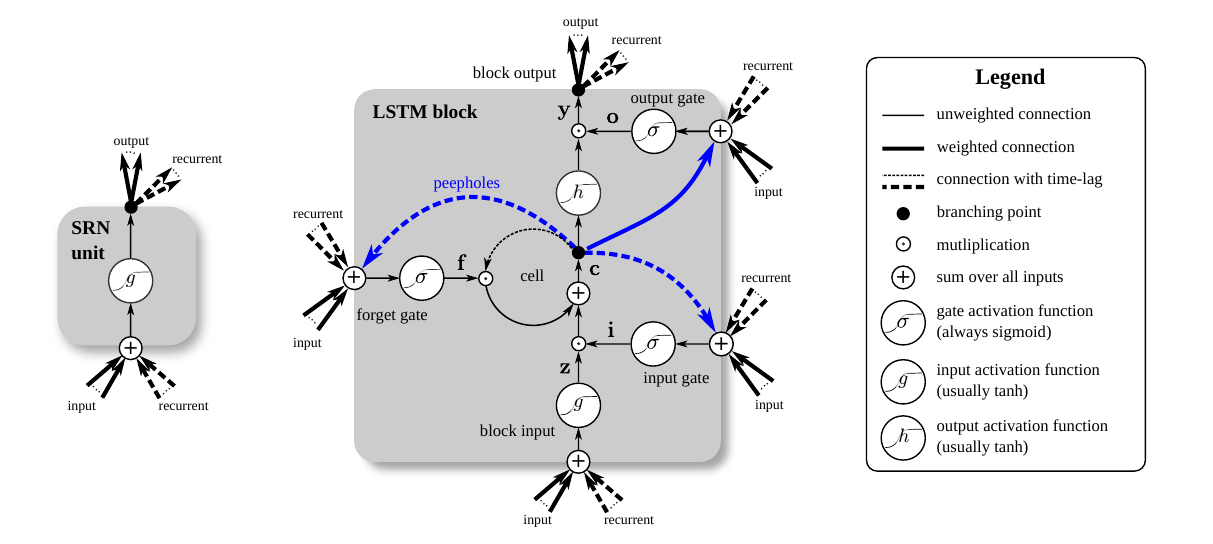
\includegraphics[width=0.9\linewidth]{figures/lstmneuron.png}
    \caption{A complete LSTM neuron, with all the features as described in~\cite{Graves05}}
	\label{fig:lstmneuron}
\end{figure}

\subsection{Training -- SPSA}\label{sec:training_lstm}
Since this work aims to perform on-chip learning, it is important to find a suitable learning scheme. Since I am aiming at an hardware implementation, and although the memory resources of nowadays FPGAs are abundant, one must find an algorithm that uses the less memory as possible (at the smallest performance cost possible), in order to use the additional memory, for instance, to add additional LSTM cells that can improve the performance of our system. 
That being said, we see that the usual training algorithms for LSTM cells -- i.e. Real-Time Recurrent Learning (RTRL), Truncated Backpropagation Through Time (BPTT) or a mixture of both~\cite{Graves05}~\cite{Hoch97}~\cite{Greff15} -- usually involve the storage of the deltas of each layer for every time instant in the training epoch (from $0$ to $T$), which is a highly non-scalable solution both in terms of memory and performance. A most efficient approach to training times series dependant structures like LSTM is the use of \textbf{Simultaneous Perturbation Stochastic Approximation} (SPSA)~\cite{Spall98}. The weight update for the $i$-th weight at the time step $t$ is given by 

\begin{equation}\label{eq:spsa_weightUpdate}
    \Delta w_i^{(t)} = \frac{J(\mb{w}^{(t)} + \beta \mb{s}^{(t)}) - J(\mb{w}^{(t)})}{\beta s_i^{(t)}}
\end{equation}
where $\beta$ is the magnitude of the perturbation to be introduced, $\mb{s}^{(t)}$ is a \textit{sign vector} whose $i$-th element, $s_i^{(t)}$, is either $-1$ or $1$. This way, we see that every weight is \textbf{randomly} incremented either by $-\beta$ or $\beta$, and we only need to keep a duplicate of the weight matrix with the perturbations, and we only need to evaluate the cost function twice per incoming sample. As for the \textit{update rule} is concerned, we have 

\begin{equation}\label{eq:spsa_updateRule}
    w_i^{(t+1)} = w_i^{(t)} - \eta \Delta w_i^{(t)}
\end{equation}
where $\eta$ is the learning rate, and $\Delta w_i^{(t)}$ is the update for the $i$-th weight evaluated in~\ref{eq:spsa_weightUpdate}.
According to the analysis performed in~\cite{Maeda05}, performing a second-order Taylor expansion at $\mb{w} = \mb{w}^{(t)}$, and taking the expected value of the equation, we get that

\begin{equation}\label{eq:spsa_gradProof}
    E(\Delta w_i^{(t)}) = \frac{\partial J(\mb{w}^{(t)})}{\partial w_i^{(t)}}
\end{equation}
that is, the weight update approximates the gradient of the cost function relative to that weight, and so the learning rule is a special form of \textit{Stochastic Gradient Descent}.

One last comment to be made concerning the update rule, is the hipothetical need for \textbf{limits} to the weight values, when the update rule exceeds $|w_{\text{max}}|$ (in that case, we set $w_i^{(t+1)} = \pm w_{\text{max}}$), which sometimes might be needed if the behaviour of the weight update is not appropriate~\cite{Maeda05}.



\chapter{State of the Art}\label{chap:stateArt}

Over the course of this chapter, I am going to present an overview of the most recent developments related to the work of this thesis, both in terms of existing dedicated hardware implementations~\ref{sec:sa_hardware}, the most relevant work in adapting suitable training algorithms to hardware~\ref{sec:sa_training} and also some of the most relevant applications of LSTM~\ref{sec:sa_apps}, which are not FPGA-based, but demonstrate how LSTM is useful by itself, and how well it competes with other Machine Learning algorithms in terms of long time-series dependences in data.

\section{LSTM Applications (non-FPGA related)}\label{sec:sa_apps} 
LSTM Networks are nowadays one of the state of the art algorithms in deep-learning, and their performance is superior to that of other kinds of RNNs and Hidden Markov Models, both of which are generally used to address the same set of problems where LSTM are employed, namely predicting and producing classification decisions from time-series data \textbf{citation needed!}. A very comprehensive description of applications can be found in one of the initial authors webpage dedicated to the subject~\footnote{\href{http://people.idsia.ch/~juergen/rnn.html}{http://people.idsia.ch/~juergen/rnn.html}}. I will now enumerate some of the bleeding edge applications of LSTM.

\begin{itemize}
    \item \textbf{Handwriting Recognition} -- and LSTM-based network~\cite{Bertolami09}, submitted by a team of the Technische Universität München, won the 2009 ICDAR Handwriting Recognition Contest, achieveing a recognition rate of up to 91\%~\cite{ICDAR09}. LSTMs have also proven to surpass HMM based models in terms of optical character recognition in printed text, as~\cite{Breuel13} suggests.

    \item \textbf{Speech Recognition} -- an architecture\cite{Graves13} proposed by Graves et al. in 2013 achieved an astonishing 17.7\% of accuracy on the TIMT Phoneme Recognition Benchmark, which up to the date is a new record. Furthermore, it has also been used for large scale acoustic modelling of speech~\cite{Sak14}.

    \item \textbf{Handwriting Synthesis} -- a comprehensive study by Graves shows, among other sequence generation tasks such as Text Prediction, the use of LSTM to produce synthetic handwriting, that looks incredibly similar to human-produced handwriting~\cite{Graves13_2}.

    \item \textbf{Translation} -- LSTM was used by Sutskever et al. (Google) to perform sequence-to-sequence translation on the WMT'14 dataset, translating English to French with a close to state of the art score~\cite{Sustkever14}.

    \item \textbf{Biomedical Applications} -- this network architecture was used in a protein homology detection scheme~\cite{Hochreiter07} using the SCOP 1.53 benchmark dataset, displaying a staggering performance when compared to other methods. Similarly, a recent article from 2015 by Sønderby et al. suggested the use of standalone LSTM and also Convolutional LSTM to perform subcellular localization of proteins, given solely their protein sequence, with an astounding accuracy of 0.902~\cite{Sonderby15}

    \item \textbf{Music Analysis and Composition} -- Lehner et al. proposed a low-latecy solution based on LSTM, suitable for real-time detection of a singing voice in music recordings~\cite{Lehner15} whose performance surpassed other baseline methods, with lower latency. 
        In terms of music transcription from audio data, there is a study that proposes the use of LSTM cells to perform a transcription of piano recordings to musical notes~\cite{Bock12}, in order to automate music transcription. The model was trained with recordings of both acoustic pianos and synthesized pianos, and the labelling was performed using an associated MIDI file for each piece that was used in the training, showing promising results. \cite{Coca13} suggests the use of LSTM to perform autonomous computer music composition, and Eck and Schmidhüber proposed LSTM to perform Blues improvisation in~\cite{Eck02}.

    \item \textbf{Video and Image Analysis} -- Vinyals et al., at Google, proposed and LSTM network for \textbf{image captioning}, preceded by a Convolutional Neural Network to apply preprocessing to the images~\cite{Vinyals14}. This way, the LSTM works as \emph{sentence generator}, that captions the images, with state of the art performance. 
        Besides image captioning, video captioning is also an interesting topic. Venugopalan et al. recently proposed a CNN + LSTM architecture to translate video sequences to natural language~\cite{Donahue14}, using the Microsoft Research Video Description Corpus as a dataset.Tthere are other similar studies that combine image and video captioning~\cite{Donahue14_2}.


\end{itemize}




\section{Hardware Implementations of LSTM}\label{sec:sa_hardware}
Hitherto, there is but one actual implementation of an LSTM network in hardware, published recently (November 2015) by Chang et al.~\cite{Chang15} in the Computing Research Repository (CoRR). It consists on the proposal of an LSTM cell architecture for dedicated hardware, targeting a Xilinx\textregistered~ Zedboard implementation. It uses a character-level language model from Andrej Karpathy, written in Lua using the Torch7 framework (the Lua calls are implemented in C, so no performance is lost).

Although the article is not clear on whether there is active learning by the ARM CPU -- the authors refer that the CPU loads the weights before operation, and that it changes them during operation, although how and why that change is done is not even clearly explained, neither mathematically nor conceptually --, \textbf{there is no on-chip learning module} in the FPGA according to the description provided. 

The implementation itself makes an extensive use of the Multiply-and-Accumulate units (MAC) of the FPGA, which since they are limited in number in the target platform, limits the number of neurons that we can deploy in parallel. The authors report a nearly 75\% usage for only 8 LSTM neurons. Although an apparently excessive number, I am left to scrutinize whether the usage of MACs is compulsory to obtain a better performance than a CPU or if it can be discarded, allowing for smaller cells. This way, we can have a layer of more neurons occupying the same area and, hopefully, the same, or even less, resources within the FPGA.

\section{Training Algorithms and Implementation}\label{sec:sa_training}
As stated in~\ref{sec:sa_hardware}, the work of~\cite{Chang15} does not feature on-chip learning at FPGA level, although there are a handful proposed solutions for it in recent literature. I will particularly look into the ones that use SPSA (see Section~\ref{sec:training_lstm}), since that is the training algorithm of choice for my proposed solution, and also to the ones that particularly apply SPSA to the training of Neural Networks. 

The SPSA algorithm was initially published by Spall in~\cite{Spall98}, and its theoretical details are outlined in Section~\ref{sec:training_lstm}. As of applications of it to the training of general Neural Networks, the earliest examples come from 1995 and 1996 on~\cite{Maeda95, Cauwen96} where SPSA is used to train a VLSI \emph{Analog} Neural Networks, a time where the memory resources of digital circuitry were limited, and so most of these structures were analog-based. Its adequacy was also established for \textbf{control problems}, such as those proposed in~\cite{Figueiredo97}, where a Time Delay Neural Network is used to control an unknown plant in a linear feedback system.

In 2005, Maeda and Wakamura published a proposed SPSA hardware implementation~\cite{Maeda05} to train an Hopfield Neural Network in an FPGA (and thus a digital system), achieving promising results in an Altera \textregistered~ FPGA. The article carefully delineates the approach taken, and also the hardware architecture designed, so it is a very good reference for the design that I will have to implement. 

Furthermore, a 2013 article by Tavear et al.~\cite{Tavear13} proposes, for the first time, using SPSA to train LSTM Neurons, although the article focuses on proving the suitability of SPSA to LSTM, and no factual hardware implementation is done or proposed. The authors simply demonstrate the suitability using conceptual arguments and by building a software model of an SPSA-trained LSTM network, and by comparing both the performance and computing speed of their model with the results achieved by Hochreiter et al. in~\cite{Hochreiter07}. Since the forward phase in both regular LSTM and SPSA-trained LSTM is the same, the computation time suffers no performance penalty whatsoever and the learning ability is preserved to a high degree, showing that SPSA is a valid alternative do BPTT and other similar and more common training schemes.

\section{Final Overview}\label{sec:overview}
As we could attest from this small literature survey, although there is already an hardware implementation os LSTM, there is still a good deal of room for improvement by adding on chip-learning to the system, and also to restric it to a smaller use of the FPGA resources, allowing it to accomodate a more complex network. Furthermore,~\cite{Tavear13} shows that, at least for that particular case, the LSTM network doesn't suffer a great performance impact from using SPSA training, as opposed to the more common BPTT, and~\cite{Maeda05} showed that an SPSA hardware implementation is feasible. These three conclusions combined indicate that the idea of a hardware LSTM network with on-chip learning using SPSA is possible. 

Besides the proposed hardware implementation, it would be advantageous to perform \emph{benchmarks} to see how well it compares with software solutions, and Section~\ref{sec:sa_apps} suggests a handful of examples to test my final solution.

\chapter{Work Plan}\label{chap:workPlan}

\section{Approach and  Main Tasks}
Dwight Eisenhower, United States' President from 1953 to 1961 and Army Officer, said that `no battle was ever won according to plan, but no battle was ever won without one'. Hence, although this initial planning draft might not be religiously followed in all its extent, it is important to break down the work in \textbf{tasks} so that I and my supervisors can keep track of what has to be done, and establishing deadlines for the small achievements that, together, will build up to the successful completion of the proposed work of this thesis. The detailed explanation of each task is provided in Section~\ref{sec:wp_tasks_td} and the \textbf{schedule} for them, where their estimated begin and end weeks are marked, is represented by a \emph{Gantt Chart} in Section~\ref{sec:wp_tasks_gantt}.

\subsection{Task Description}\label{sec:wp_tasks_td}
The work will be partitioned in \emph{five} large groups of tasks, and each of these groups will be further partitioned in smaller subtasks which are the actual assignments that I will be completing. We can think of the group of task as a sort of \emph{logical} grouping of the subtasks, according both to their relatedness and also to their precedence relationships. The task groups, and their related subtasks, are as follows:

\begin{itemize}
    \item \textbf{T1 -- Preparation} -- This stage is the initial phase of the work, where I will essentially setup my working environment and finish the Python modules for the LSTM network that will be used in the validation of my Verilog modules

        \begin{itemize}
            \item \textbf{T1.1 -- Complete Python Implementation with SPSA} -- here I will finish the Python modules that I have already developed as a preparation for this work, whose details are presented in Section~\ref{chap:earlyWork}, by adding the SPSA training algorithm, as opposed to the current Backpropagation Through Time version.

            \item \textbf{T1.2 -- Reproduce the Benchmark Results with the Python Implementation} -- after developing and testing the Python Class with SPSA, I will try to reproduce with it the results of~\cite{Tavear13}, in order for me to have a high-level model whose performance is comparable to~\cite{Tavear13, Hochreiter07}, and thus provide a good performance baseline for this and other future benchmark tests that I would like to run in order to compare my FPGA solution with a software solution.

            \item \textbf{T1.3 -- Setup FPGA Development Board} -- this is a fairly technical step, where I setup my working environment, and make sure that everything is working correctly and is properly configured. As will be pointed out in Section~\ref{sec:wp_sh}, the FPGA development board of choice will be Xilinx~\textregistered Zedboard.

            \item \textbf{T1.4 -- Familiarize with the Zedboard} -- before any actual use, I should synthesize and run some sample designs, and perhaps write a small Verilog design, and go through the full design flow, from behavioural simulation, to synthesis. This will allow me to know exactly what steps to take when I will need to develop and test my Dissertation related modules, and focus more on the solving the problem at hand rather than solving technical details.
        \end{itemize}

    \item \textbf{T2 -- HDL Module Development} -- this is where I will port the ideas from Section~\ref{chap:theorBack} to fully functional HDL blocks, using Verilog and targeting a Zedboard technology.

        \begin{itemize}
            \item \textbf{T2.1 -- Design Planning} -- before performing and HDL coding, it is desirable first assemble the system design strategy in paper. This is where, together with my supervisor, I will outline the internal organization of my system, and make the fundamental design decisions. Of course, this task will continue during the entire of \textbf{T2} extent, since some design changes to the original plan will have to be performed as I find \emph{bugs} in my early Verilog implementations that force a design correction.

            \item \textbf{T2.2 -- Design SPSA Module} -- this task comprises the Verilog description of the module that will update the network weights using SPSA, and also the development of a testbench to validate my description. Furthermore, I will compare the output of this model with the golden output produced by a standalone SPSA Python Class previously developed in \textbf{T1}.

            \item \textbf{T2.3 -- Design LSTM Neuron/Layer Module} -- similarly to the previous task, but now I am aiming to implement the actual LSTM Neuron or a layer of LSTM Neurons. This is a design decision that will need to be set in \textbf{T2.1}, to assess whether it is justifiable to have dedicated multiplication units assigned to each neuron, or we can perform matrix-like batch multiplications and treat the LSTM as a batch of Neurons, i.e. as a layer. Like in the previous task, a testbench will also be developed, and the module validate both with it and the Python golden output.

            \item \textbf{T2.4 -- Integrate and Validate both LSTM and SPSA modules} -- here, after the modules designed in \textbf{T2.2} and \textbf{T2.3} are validated individually, I will integrate them together in a higher level module, and perform a behavioural simulations of the new integrated module, as well as a verification procedure where the results from~\cite{Tavear13} will hopefully be reproduced and compared against the Python golden output.

        \end{itemize}

    \item \textbf{T3 -- FPGA Synthesis of the Verilog Code} -- after having Verilog code that passed all the validation tests and whose correct functionality is, therefore, ensured, I will synthesize the Verilog modules to FPGA RTL blocks, and perform a new simulation on these RTL syntesized code, that unlike the previous behavioural simulation, now has timing information resulting from the FPGA block mapping, and the place and routing of those mapped blocks.

        \begin{itemize}
            \item \textbf{T3.1 -- Synthesis of the SPSA Module} -- the module developed in \textbf{T2.2} is now synthesized and validated.
            \item \textbf{T3.2 -- Synthesis of the LSTM Neuron/Layer Module} -- same as the previous task, but now on the module of \textbf{T2.3}
            \item \textbf{T3.3 -- Integration of the Modules and Validation} -- the modules synthesized in the previous tasks are integrated and validated using the same testbench as in \textbf{T2.4}.
        \end{itemize}

    \item \textbf{T4 -- Benchmarking the Design} -- at this stage, we have a fully functional FPGA design of an LSTM network with SPSA on-chip training. Henceforth, we will need to benchmark its performance by comparing it to~\cite{Tavear13, Hochreiter07}, and prove its usefulness by using it in one or two use-cases from~\ref{chap:stateArt}, which are interesting uses of Deep Learning techniques such as these.

        \begin{itemize}
            \item \textbf{T4.1 -- Benchmark the Performance/Computing Time} -- perform a side-by-side comparison of our model with the software counterpart of~\cite{Tavear13, Hochreiter07} and with the only hardware implementation of LSTM of~\cite{Chang15}.
            \item \textbf{T4.2 -- Reproduce some of the state of the art applications of LSTM} -- in order to be able to show real-life, user-oriented, applications, I understand it is a good idea to try to reproduce some of the state of the art usages of LSTM, outlined in Section~\ref{sec:sa_apps}. It is too early to commit myself to which of these applications I will use, and how many, because that will depend on how well the work on tasks \textbf{T2} and \textbf{T3} is flowing. Nevertheless, I intend to at least implement one or two of them.
        \end{itemize}

    \item \textbf{T5 -- Write the Dissertation Final Report} -- while all the stages of work are progressing, this task will obviously be active, by documenting all the design decisions, milestones achieved and logging all the results that come from the implementation. A couple of weeks before the deadline, this will be the only active task, since producing a clear and well-written document requires concentration and undivided attention.

\end{itemize}

\subsection{Tentative Task Scheduling}\label{sec:wp_tasks_gantt}
Here is the Gantt Chart that depicts the temporal extension of the tasks described in Section~\ref{sec:wp_tasks_td}. 
\begin{landscape}
    
    \ganttset{bar height=.2}
    \ganttset{calendar week text= \small {\startday/\startmonth}}
    \begin{ganttchart}[vgrid, x unit=0.16cm, y unit chart=0.65cm, time slot format=isodate]{2016-02-15}{2016-06-26}

        \gantttitlecalendar{year, month, week} \\
        \ganttgroup{\textbf{T1}}{2016-02-15}{2016-02-29} \\
        \ganttbar{\textbf{T1.1}}{2016-02-15}{2016-02-22} \\
        \ganttbar{\textbf{T1.2}}{2016-02-22}{2016-02-29} \\
        \ganttbar{\textbf{T1.3}}{2016-02-15}{2016-02-22} \\
        \ganttbar{\textbf{T1.4}}{2016-02-22}{2016-02-29} \\

        \ganttgroup{\textbf{T2}}{2016-02-29}{2016-04-11} \\
        \ganttbar{\textbf{T2.1}}{2016-02-29}{2016-03-28} \\
        \ganttbar{\textbf{T2.2}}{2016-02-29}{2016-03-07} \\
        \ganttbar{\textbf{T2.3}}{2016-03-07}{2016-03-21} \\
        \ganttbar{\textbf{T2.4}}{2016-03-21}{2016-04-11} \\
        
        \ganttgroup{\textbf{T3}}{2016-04-11}{2016-05-02} \\
        \ganttbar{\textbf{T3.1}}{2016-04-11}{2016-04-18} \\
        \ganttbar{\textbf{T3.2}}{2016-04-18}{2016-04-25} \\
        \ganttbar{\textbf{T3.3}}{2016-04-25}{2016-05-02} \\

        \ganttgroup{\textbf{T4}}{2016-05-02}{2016-06-06} \\
        \ganttbar{\textbf{T4.1}}{2016-05-02}{2016-05-16} \\
        \ganttbar{\textbf{T4.2}}{2016-05-09}{2016-06-06} \\

        \ganttgroup{\textbf{T5}}{2016-02-29}{2016-06-26} \\

    \end{ganttchart}

\end{landscape}
\section{Software and Hardware resources to be used}\label{sec:wp_sh}

\subsection{Hardware Resources}
The main hardware resource that I will use for my solution is the \textbf{Xilinx\textregistered~ Zedboard} (Figure~\ref{fig:zedboard}), whose core is a Zynq-7000 System-on-Chip that features both an FPGA core and two ARM \textregistered~ Cortex\texttrademark~-A9 processors. It is an FPGA development board that features several I/O interfaces such as Ethernet, HDMI output, VGA output, Audio IOs, USB and UART, among other capabilities, making it easy to prototype additional features to the core design (i.e. for building the note transcription system of~\cite{Bock12}, and to make it operate in real-time, I would need an audio input, which I can easily get from the Audio IO, without investing time in connecting the codec and programming the FPGA to interface it).

\begin{figure}
    \centering
    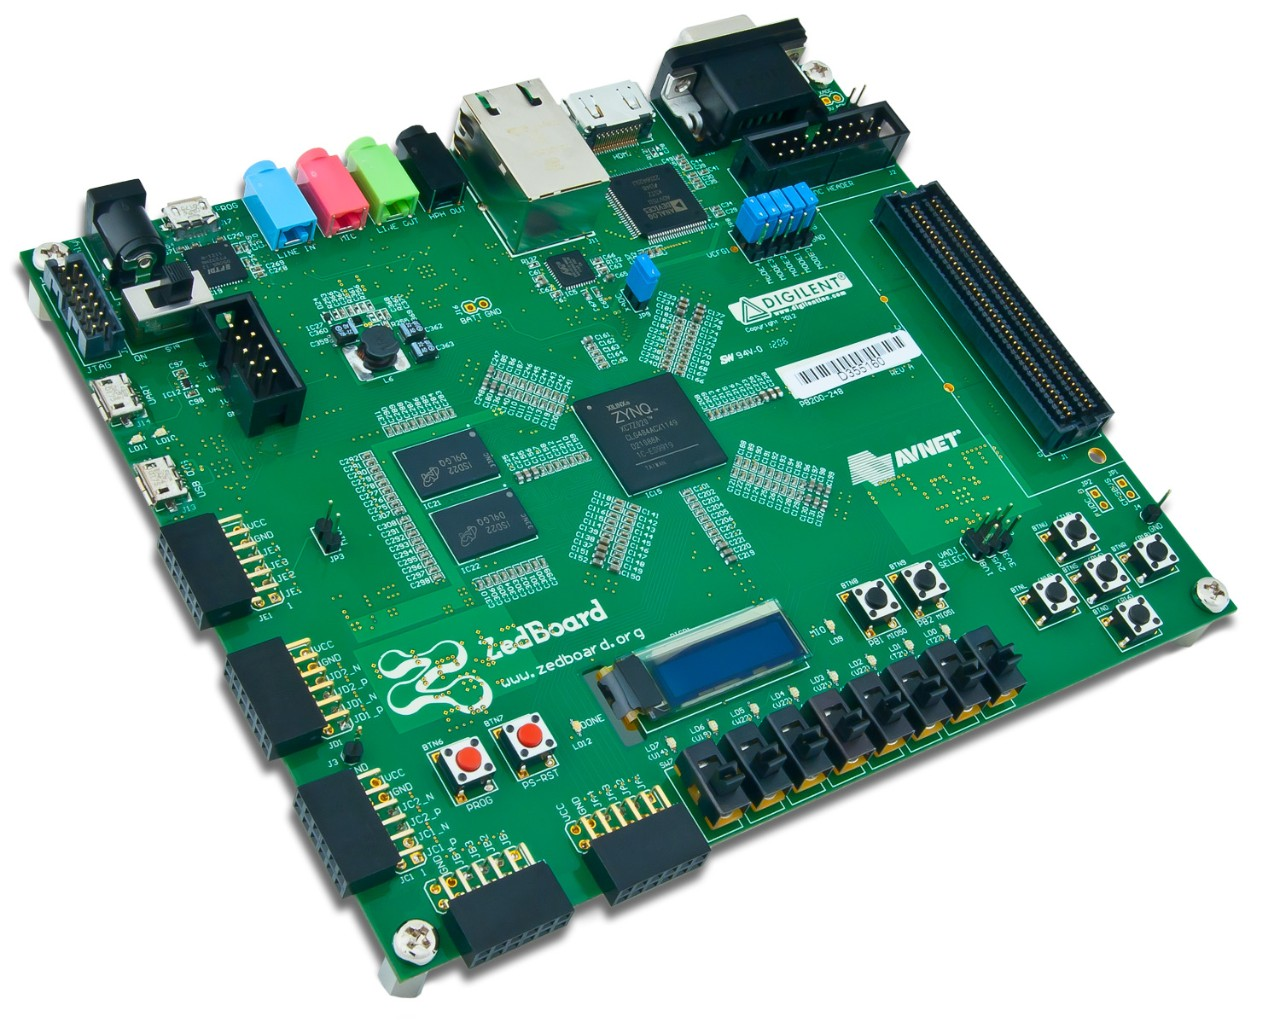
\includegraphics[width=\linewidth]{figures/zedboard.jpg}
    \caption{The Zedboard FPGA Development Board. Source: \href{http://www.xilinx.com}{Xilinx}}
    \label{fig:zedboard}
\end{figure}

\subsection{Software Resources}
In terms of software resources related to the FPGA development, I will need an \textbf{HDL simulation tool} to simulate and verify the Verilog code that I will develop, and a \textbf{Synthesis tool} to synthesize the Verilog files into RTL code, and to map that description into the resources available in the FPGA. The simulation tool used will be Questasim\texttrademark, the successor of the well-known Modelsim\texttrademark, which is an industry-standard tool in the area. For the synthesis tool, I will use Xilinx\textregistered Vivado Suite, also an industry-standard tool, and that is the only alternative, since the Zedboard is also produced by Xilinx\textregistered. These two tools are proprietary, but there are licenses available at FEUP. Furthermore, I am planning to use FloPoCo~\footnote{\href{http://flopoco.gforge.inria.fr/}{http://flopoco.gforge.inria.fr/}} to generate some of the modules that perform arithmetic operations, to hasten the developing effort/time, and to ensure that they are the most efficient possible, and don't pose a performance bottleneck to my design; this software is freeware, and a standard in Academia.

For the Python implementation, I will make use of the 3.3 version of the Python distribution, the high-performance numerical computation library Numpy\footnote{\href{http://www.numpy.org/}{http://www.numpy.org/}}, which is a standard in scientific computing, and the Matplotlib\footnote{\href{http://matplotlib.org/}{http://matplotlib.org/}} plotting library. All of this software is also free to use, and open-source. I may also need to use the PyBrain\footnote{\href{http://pybrain.org/}{http://pybrain.org/}} framework, since it has an LSTM implementation. 

To write the final Dissertation report, I will use \LaTeX~(this report itself was also written in \LaTeX), and mostly use Tikz, Inkscape and Matplotlib to produce figures and drawings. Once again, all of these are free to use.

\chapter{Early Work}\label{chap:earlyWork}
In order to better undesrtand LSTM,  gain some useful insight on their operation, and to have a software implementation, that is not part of any framework, with which I can validate in the future my FPGA implementation, I have developed a fully functional LSTM Layer in Python and Numpy, that still uses BPTT as a training algorithm (the governing equations are in appendix A of~\cite{Greff15}). The idea is to adapt it to use SPSA in the beginning of my Master's work. The code is present in

\lstinputlisting[language=Python, caption=Implementation of a LSTM Layer]{LSTMlayer.py}


%% comment next 2 commands if numbered appendices are not used
\appendix
\chapter{Loren Ipsum} \label{ap1:loren}

Depois das conclusões e antes das referências bibliográficas,
apresenta-se neste anexo numerado o texto usado para preencher a
dissertação.

\section{O que é o \emph{Loren Ipsum}?}


\section{De onde Vem o Loren?}


%%----------------------------------------
%% Final materials
%%----------------------------------------

%% Bibliography
%% Comment the next command if BibTeX file not used
%% bibliography is in ``myrefs.bib''
\PrintBib{bibliography}
%\bibliographystyle{IEEETran}
%\bibliography{bibliography}
%% Index
%% Uncomment next command if index is required
%% don't forget to run ``makeindex thesis'' command
%\PrintIndex

\end{document}
